% !TeX root = ../Main/XMU.tex
\chapter{方法}{Methodology}
在本节中,将会完整阐述本文提出的基于监督学习方法的IK解算器。 \cref{fig:flowchart}说明了我们方法的整体流程。 我们方法的关键组件是Motion Predictor(MP)和Posture Estimator(PE)。前者根据当前运动轨迹来预测末端效应器的未来位置,而后者基于一系列末端效应器位置估计身体姿势。
\begin{figure}[!h]
	\centering
	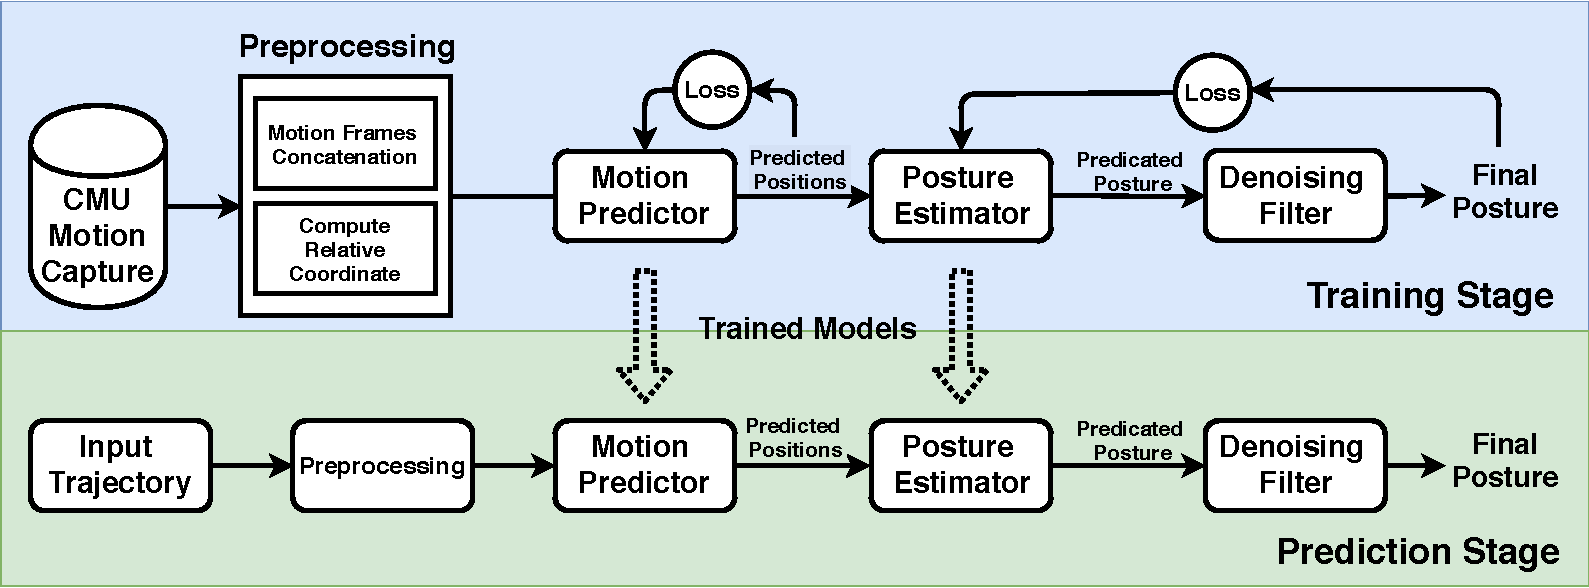
\includegraphics[width=\linewidth]{flowchart}
	\caption[]{\label{fig:flowchart}
		本方法的流程图
	}
\end{figure}

首先对本文中使用的一些术语进行定义:
\begin{itemize}
\item\textbf{骨骼(skelton)}骨骼$\mathbf{S}$定义具有根关节及其相互连接的关节角色的层次结构,而关节距离适用于构造具有几何变量的角色。
\item\textbf{末端执行器(end-effector)}末端执行器$\mathbf{EE}$通常指与环境进行交互的角色的脚和手。
\item\textbf{姿态(posture)}姿态$\mathbf{P}$是描述角色身体结构的向量,由根关节的全局变换和关节方向的角度值组成。
\item\textbf{动作(motion)}动作$\mathbf{M}$是一个矩阵,用于描述时域中的一系列角色姿势。矩阵行数对应帧数,列数与关节通道数成比例。
\item\textbf{位置(position)}位置$\mathbf{PE}$描述$\mathbf{EE}$的全局位置。
\item\textbf{正向运动学(forward kinematics)}指的是在给定特定角色姿势的3D空间中计算末端效应器位置的过程。
\item\textbf{逆向运动学(inverse kinematics)}
指的是当已知末端执行器放置在所需目标位置时,计算沿身体骨骼连接的关节方向的过程。
\end{itemize}

\section{离线网络学习}{Offline Network Learning}
\subsection{数据集和预处理}{Datasets and Preprocessing}
本项工作使用Carnegie Mellon University(CMU)的Mocap数据库来构建此问题中的神经网络的训练集和测试集。 训练数据集包含约2000个动作序列(约200万个骨骼姿势),而测试数据集包含约200个动作序列(约20万个骨骼姿势)。构建训练集和测试集时,使用正向运动学技术来计算骨骼关节的世界坐标位置。 我们提出了一种分层结构,它由四个独立的IK解算器组成,分别用于计算左/右臂和左/右腿。

我们定义了两种有效的技巧用来提高神经网络的学习性能:

\textbf{建立连续帧之间的时间关联性}实验证明,将连续的多帧的运动序列$[\cdots, X_{t-2*k}, X_{t-k},$ $ X_{t}, X_{t+k}, X_{t+2*k},\cdots]$替代传统的以末端执行器的当前位置作为网络输入在提高预测精度方面是有效的。 这在我们的实验中得到了证实。\textcolor{red}{见图7和相关章节}。

\textbf{运用肩关节-腕关节/髋关节-踝关节的相对坐标}在本项工作中,通过计算肩关节-腕关节和髋关节-踝关节的相对向量来表示手臂和腿部的末端效应器的当前位置。采取这样的近似处理基于以下假设:股骨:胫骨和肱骨:尺骨的比例在个体之间的差异非常小。这样的处理也允许训练完毕后的IK解算器能够适应具有不同几何长度和几何形状的的角色。

通过这些技巧,我们可以构建神经网络监督学习中\*X和\*Y之间的映射:

\begin{itemize}
\item $\mathbf{X}$:向量$N_X$表示从分层骨骼结构和动作联合通道中帧序列中末端效应器的全局位置。
\item $\mathbf{Y}$:向量$N_Y$表示身体各个关节方向的旋转角度值。训练集和测试集中的该值直接从动作文件的相应通道进行复制。后续的操作中,为了提高神经网络的训练过程的表现,对该值做了数学方法的处理,但不改变该值的原始定义和所表达的意义。
\end{itemize}

\subsection{IK解算器关键组件}{Main Components of IK Solver}

Motion Predictor($\mathbf{MP}$)和Posture Estimator($\mathbf{PE}$)MP和PE是我们IK解算器的两个主要组成部分,我们使用相同的神经网络结构来构建这两个组件。 该网络的主体是递归神经网络(RNN),具有三层LSTM(每层的大小为512),随后是全连接层。

\textcolor{red}{补充一张网络模型图}

$\mathbf{MP}$组件所用的神经网络的输入是过去$\mathbf{K}$帧中的$\mathbf{EE}$位置序列,输出是下一个$\mathbf{K}$K帧中的$\mathbf{EE}$位置序列。 神经网络的损失函数定义为:
\begin{equation}
L_m = \sum_{i=0}^{K_m} (\mathbf{PE}_i - \mathbf{PE}_i^G)
\end{equation}
该式中,$K_m$表示连续帧的帧数,$\mathbf{PE}_i^G$表示来自运动捕捉数据库的真实值.

$\mathbf{PE}$组件所用的神经网络的输入是过去$\mathbf{K}$帧中$\mathbf{EE}$和下一个$\mathbf{K}$帧中的位置序列,输出是过去$\mathbf{K}$帧中和下一个$\mathbf{K}$帧中的$\mathbf{EE}$预测姿势序列。 神经网络的损失函数定义为:
\begin{equation}
L_p = \sum_{i=0}^{K_p} (\mathbf{P}_i - \mathbf{P}_i^G)
\end{equation}
该式中,$K_p$表示连续帧的帧数,$\mathbf{P}_i^G$表示来自运动捕捉数据库的真实值。

\textbf{优化器、优化算法和超参数}深度神经网络采用目前流行的RNN网络模型作为网络连接模式以适用连续帧之间的时间关联性,选用ReLU作为激活函数、Adam优化器作为优化函数。网络的超参数为:$batch size=128$,$learning_rate=0.0001$,$maximal epoch = 1000$.

\textbf{网络参数调节}
在实际的训练过程中,为达到最好的训练效果,在模型的参数上和样本集的处理可能会做一些微调以达到更好的精度和更快的训练速度:
\begin{itemize}
\item{学习率下降(learning rate decay)}防止学习率过大,在收敛到全局最优点的时候会来回摆荡,所以学习率随着训练轮数不断按指数级下降,收敛梯度下降的学习步长。

\item{梯度剪切(weithts regularization)}训练集的规模的约束导致了神经网络的层数在设计过程中需要比过往经验中的更多。正因如此,梯度爆炸和梯度消失的现象有可能在网络模型的参数调整过程中出现。为了解决这一问题,设计一个梯度阈值,如果超过该阈值,直接将梯度置为该值。
\end{itemize}

\textbf{去噪滤波器}\textbf{PE}网络的输出存在一定的噪音(连续帧之间动作不够平滑,即视觉上骨骼轻微抖动)进一步使用平均滤波器进行处理以进行去噪。平均滤波器的处理过程如下:
\begin{equation}
\mathbf{P} = \frac{1}{N} \sum_i^k {\mathbf{P}_i}
\end{equation}
$\mathbf{P}_i$示\textbf{PE}网络输出的连续预测姿势序列.

这一步显著提高了\textbf{PE}输出预测姿势序列的平滑度。

\section{姿态综合和姿势估计}{Posture Synthesis and Estimation}

本项工作的IK求解器应用于两个应用:姿势合成和姿态估计。
\begin{itemize}
\item{\textbf{姿势合成}}在用户指定末端执行器的轨迹后,以0.5秒的均匀间隔对轨迹进行采样,然后自动生成全身姿势。轨迹的生成由两个步骤组成:相对坐标的计算和运动帧级联。预测程序的流程如\cref{flowchart}所示。
\item{\textbf{姿态估计}}本项工作着重于解决使用2D单人图像到3D人体骨骼姿态的估计。由于这是一个典型的不适定问题,所以解决该问题时具有一定的挑战性。在实际的应用中,对于每个人体几何信息进行采集几乎是不可能的,所以本文所涉及的工作中,仅使用由2D图像到3D骨骼预测流程中输出的$\mathbf{EE}$的3D位置和与其对应的根关节位置,并应用本文提出的IK解算器对当前身体骨骼连接做出一个最佳姿态的估计。
\end{itemize}












